\documentclass[a4paper, 12pt]{article}

\usepackage[spanish]{babel}
\usepackage[utf8]{inputenc}
\usepackage{amsmath}
\usepackage{graphicx}
\usepackage{a4wide}

\title{Examen Métodos Numéricos I \\ 2ª Semana Febrero 2013}
\author{Unai Aguilera Irazabal DNI: 45663055-M}
\date{13 de febrero de 2013}

\begin{document}
\maketitle

\section*{Problema 1}
\subsection*{Eliminación gaussiana}
A partir del sistema de ecuaciones se construye la matriz aumentada de
coeficientes del sistema.

\begin{align*}
\begin{pmatrix}
  4 & 1 & 1 & 4\\
  1 & 4 & -2 & 4 \\
  3 & 2 & -4 & 6
\end{pmatrix}
\end{align*}

A partir de ella se aplica el proceso de eliminaciones para convertir la 
matriz en una matriz triangular superior.

\begin{align*}
\begin{pmatrix}
  4 & 1 & 1 & 4\\
  1 & 4 & -2 & 4 \\
  3 & 2 & -4 & 6
\end{pmatrix} 
\xrightarrow[R_3 = -\frac{3}{4}R_1 + R_3]{R_2 = -\frac{1}{4}R_1 + R_2}
\begin{pmatrix}
  4 & 1 & 1 & 4\\
  0 & 15/4 & -9/4 & 3 \\
  0 & 5/4 & -19/4 & 3
\end{pmatrix}
\end{align*}

\begin{align*}
\xrightarrow{R_3 = -\frac{1}{3}R_2 + R_3}
\begin{pmatrix}
  4 & 1 & 1 & 4\\
  0 & 15/4 & -9/4 & 3 \\
  0 & 0 & -4 & 2
\end{pmatrix}
\end{align*}

Ahora se aplica una substitución hacia atrás para obtener los valores de las
incógnitas

\begin{align*}
-4I_3 = 2
\rightarrow
I_3 = -\frac{1}{2}
\end{align*}

\begin{align*}
\frac{15}{4}I_2 - \frac{9}{4}I_3 = 3 
\rightarrow
\frac{15}{4}I_2 - \frac{9}{4}(-\frac{1}{2}) = 3
\rightarrow
I_2 = \frac{1}{2}
\end{align*}

\begin{align*}
4I_1 + I_2 + I_3 = 4 
\rightarrow
4I_1 + (\frac{1}{2}) + (-\frac{1}{2}) = 4
\rightarrow
I_1 = 1
\end{align*}

\subsection*{Método de reducción de Crout}
Se plantea la descomposición LU de la matriz de coeficientes A de tal forma que

\begin{align*}
\begin{pmatrix}
  l_{11} & 0 & 0\\
  l_{21} & l_{22} & 0\\
  l_{31} & l_{32} & l_{33}
\end{pmatrix} 
\begin{pmatrix}
  1 & u_{12} & u_{13}\\
  0 & 1 & u_{23}\\
  0 & 0 & 1
\end{pmatrix}
=
\begin{pmatrix}
  a_{11} & a_{12} & a_{13}\\
  a_{21} & a_{22} & a_{23}\\
  a_{31} & a_{32} & a_{33}
\end{pmatrix}
\end{align*}

Al multiplicar las filas de L por la primera columna de U se obtiene que
\begin{align*}
l_{11} = 4;~~~
l_{21} = 1;~~~
l_{31} = 3;~~~
\end{align*}

ahora, al multiplicar la primera fila de L por las columnas de U
\begin{align*}
u_{12} = \frac{a_{12}}{l_{11}} = \frac{1}{4};~~~
u_{13} = \frac{a_{13}}{l_{11}} = \frac{1}{4};~~~
\end{align*}

posteriormente se multiplican las filas de L por la segunda columna de U
\begin{align*}
l_{22} = a_{22} - l_{21}u_{12} = 4 - 1\frac{1}{4} = \frac{15}{4}\\
l_{32} = a_{32} - l_{31}u_{12} = 2 - 3\frac{1}{4} = \frac{5}{4}
\end{align*}

la segunda fila de L por las columnas de U
\begin{align*}
u_{23} = \frac{a_{23}}{l_{23}u_{13}} =
\frac{-2 - 1\frac{1}{4}}{\frac{15}{4}} = -\frac{3}{5}
\end{align*}

y finalmente, las filas de L por la tercera columna de U
\begin{align*}
l_{33} = a_{33} - l_{31}u_{13} - l_{32}u_{23} =
-4 - 3\frac{1}{4} - \frac{5}{4}(-\frac{3}{5}) = -4
\end{align*}

Se obtiene así la siguiente descomposición LU de la matriz A
\begin{align*}
\begin{pmatrix}
  4 & 0 & 0\\
  1 & 15/4 & 0\\
  3 & 5/4 & -4
\end{pmatrix} 
\begin{pmatrix}
  1 & 1/4 & 1/4\\
  0 & 1 & -3/5\\
  0 & 0 & 1
\end{pmatrix}
=
\begin{pmatrix}
  4 & 1 & 1\\
  1 & 4 & -2\\
  3 & 2 & -4
\end{pmatrix}
\end{align*}

Ahora se amplía la matriz L con la columna de términos independientes del
sistema

\begin{align*}
\begin{pmatrix}
  4 & 0 & 0 & 4\\
  1 & 15/4 & 0 & 4 \\
  3 & 5/4 & -4 & 6
\end{pmatrix}
\end{align*}

y se realiza una substitución hacia delante para transformar los terminos
independientes

\begin{align*}
4b_1 = 4
\rightarrow
b_1 = 1
\end{align*}

\begin{align*}
b_1 + \frac{15}{4}b_2 = 4 
\rightarrow
1 + \frac{15}{4}b_2 = 4
\rightarrow
b_2 = \frac{12}{15}
\end{align*}

\begin{align*}
3b_1 + \frac{5}{4}b_2 + 4b_3 = 6 
\rightarrow
3 + \frac{5}{4}(\frac{12}{15}) + 4b_3 = 6
\rightarrow
b_3 = -\frac{1}{2}
\end{align*}

Utilizando dichos términos transformados para ampliar la matriz U

\begin{align*}
\begin{pmatrix}
  1 & 1/4 & 1/4 & 1\\
  0 & 1 & -3/5 & 12/15 \\
  0 & 0 & 1 & -1/2
\end{pmatrix}
\end{align*}

y de donde realizando una substicución hacia atrás se obtienen los valores de
las incógnitas
\begin{align*}
I_3 = -\frac{1}{2}
\end{align*}

\begin{align*}
I_2 - \frac{3}{5}I_3 = \frac{12}{15} 
\rightarrow
I_2 - \frac{3}{5}(-\frac{1}{2}) = \frac{12}{15}
\rightarrow
I_2 = \frac{1}{2}
\end{align*}

\begin{align*}
I_1 + \frac{1}{4}I_2 + \frac{1}{4}I_3 = 1 
\rightarrow
I_1 + \frac{1}{4}(\frac{1}{2}) + \frac{1}{4}(-\frac{1}{2}) = 1 
\rightarrow
I_1 = 1
\end{align*}

\section*{Problema 2}
Para aplicar la cuadratura gaussiana a 

\begin{equation*}
	\int^{1}_{0} x e^{-x^2} dx
\end{equation*}

es necesario cambiar el intervalo de integración a (-1, 1). Para ello se aplica
el siguiente cambio de variable

\begin{equation*}
x = \frac{(b - a)t + b + a}{2} = \frac{(1 - 0)t + 1 + 0}{2} = \frac{t + 1}{2}
\end{equation*}

\begin{equation*}
dx = \frac{b - a}{2} = \frac{(1 - 0)}{2} = \frac{1}{2}
\end{equation*}

\begin{equation*}
	\int^{1}_{0} x e^{-x^2} dx =
	\frac{1}{4}\int^{1}_{-1} (t + 1) e^{-\frac{(t + 1)^2}{4}} dx
\end{equation*}

El valor de la integral obtenido de manera analítica es

\begin{equation*}
  \int^1_0 x e^{-x^2} = -\frac{1}{2} \int^{-1}_0 e^z dz =
  -\frac{1}{2} e^z|^{-1}_{0} = \frac{1}{2}(1-\frac{1}{e}) = 0.316060
\end{equation*}

Los valores obtenidos al aplicar la cuadratura para $n=1,2,3,4$
\begin{itemize}
\item $n=1$:\\
$\frac{1}{4}[(2.0)((0.0 + 1) e^{-\frac{(0.0 + 1)^2}{4}})] = 0.389400$\\
$e_r=0.232045$ 
\item $n=2$:\\ 
$\frac{1}{4}[(1.0)((-0.57735027 + 1) e^{-\frac{(-0.57735027 + 1)^2}{4}}) +\\ 
(1.0)((0.57735027 + 1) e^{-\frac{(0.57735027 + 1)^2}{4}})] = 0.312754$\\
$e_r=0.010462$
\item $n=3$:\\
$\frac{1}{4}[(0.55555555)((-0.77459667 + 1) e^{-\frac{(-0.77459667 + 1)^2}{4}}) +\\ 
(0.888888889)((0.0 + 1) e^{-\frac{(0.0 + 1)^2}{4}}) +\\
(0.55555555)((-0.77459667 + 1) e^{-\frac{(-0.77459667 + 1)^2}{4}})] = 0.234889$\\
$e_r=0.256823$
\item $n=4$:\\
$\frac{1}{4}[(0.34785485)((-0.86113631 + 1) e^{-\frac{(-0.86113631 + 1)^2}{4}}) +\\ 
(0.65214515)((-0.33998104 + 1) e^{-\frac{(-0.33998104 + 1)^2}{4}}) +\\
(0.65214515)((0.33998104 + 1) e^{-\frac{(0.33998104 + 1)^2}{4}}) +\\
(0.34785485)((0.86113631 + 1) e^{-\frac{(0.86113631 + 1)^2}{4}})] = 0.259994$\\
$e_r=0.177390$
\end{itemize} 

\section*{Problema 3}
Como en la aproximación de Padé pedida el grado del numerador y el denominador
es 2, se necesita calcular primeramente la aproximación de McLaurin de grado
$N = m + n = 4$. Así,
\begin{equation*}
 f_{M4}(x) = 2 + x^2 + \frac{x^4}{12}
\end{equation*} 

Por otro lado, la aproximación de Padé se construye como
\begin{equation*}
R_4(x) = \frac{a_0 + a_1x + a_2x^2}{1 + b_1x + b_2x^2}
\end{equation*} 

Se define la diferencia de las dos ecuaciones anteriores
\begin{align*}
f_{M4}(x) - R_4(x) = (2 + x^2 + \frac{x^4}{12}) -
                    \frac{a_0 + a_1x + a_2x^2}{1 + b_1x + b_2x^2} =\\
                    \frac{(2 + x^2 + \frac{x^4}{12})(1 + b_1x + b_2x^2) - (a_0 + a_1x + a_2x^2)}{1 + b_1x + b_2x^2}
\end{align*}

Es necesario seleccionar las constantes $a_0, a_1, a_2, b_1, b_2$ para que se
cumpla
\begin{equation*}
 f_{M4}^{(k)}(0) - R_4^{(k)}(0) = 0, ~~~para~~~k = 0, 1, ..., N
\end{equation*}

La condición anterior es equivalente a que en la función resta se anulen todos
los coeficientes para menores que $N=4$. Se obtienen las siguientes ecuaciones
\begin{align*}
2 - a_0 = 0\\
2b_1 - a_1 = 0\\
2b_2 + 1 - a_2 = 0\\
b_1 = 0\\
b_2 = 0
\end{align*}
de donde se obtiene que $a_0 = 2, a_1 = 0, b_1 = 0, b_2 = 0$ y, por lo tanto,
la aproximación de Padé pedida es
\begin{equation*}
R_4(x) = \frac{2 + x^2}{1}
\end{equation*}

El valor analítico de la función $f(x)$, y los errores relativos de las
aproximaciones son
\begin{align*}
f(0.1) = e^{0.1} + e^{-0.1} = 2.010008\\
f_{M4}(x) = 2 + 0.1^2 + \frac{0.1^4}{12} = 2.010008~~~e_r=0\\
R_4(x) = 2 + 0.1^2 = 2.010000~~~e_r = 4 \cdot 10^{-6}
\end{align*}

\section*{Problema 4}
El método de Euler modificado comienza estimando un valor provisional para la
función $y(t+dt)$ usando la ecuación de la derivada. Así
\begin{equation*}
 y_{n+1} = y_n + hy^{'}_n
\end{equation*}  
Esta estimación se utiliza para obtener el valor de la derivada de la función
en dicho punto $y^{'}_{n+1}$. A partir de los valores de la derivada al inicio
y final del intervalo se obtiene la media aritmética de la pendiente de la
función. Este valor mejorado para la pendiente es el realmente utilizado para
obtener el siguiente paso de la función.
\begin{equation*}
y_{n+1} = y_n + h\frac{y^{'}_{n+1} + y^{'}_{n}}{2}
\end{equation*}

En la tabla \ref{tab:resultados} se representan los valores anteriores para cada
paso de la integración hasta $t=0.5$ con $h=dt=0.1$, utilizando la condición
inicial $y(t = 0) = 1$ para comenzar el proceso. En la figura \ref{fig:grafica}
se representa la función $y(t)$ para valores $ 0 \leq t \leq 20$.
Como puede observarse median inspección visual, el periodo de la función es
apróximanadamente 6 radianes.

\begin{table}
\begin{center}
\begin{tabular}{|c|c|c|c|c|c|c|c|c|}
\hline
 t & $y(t)$ & $y^{'}_n(t)$ & $hy^{'}_n(t)$ & $y_{n+1}$ & $y^{'}_{n+1}(t+h)$ & $\frac{y^{'}_{n+1}(t+h) + y^{'}_{n}(t)}{2}$
 & $h \cdot p_{m}$ & $y(t+h)$\\
 \hline\hline
0.0  &  1.0000  &  0.5403  &  0.0540  & 1.0540  &  0.4267   & 0.4835   &  0.0483  &  1.0483\\ \hline
0.1  &  1.0483  &  0.4298  &  0.0430  &  1.0913 &   0.3010  &  0.3654  &   0.0365 &   1.0849\\ \hline
0.2  &  1.0849  &  0.3060  &  0.0306  &  1.1155 &   0.1725  &  0.2393  &   0.0239 &   1.1088\\ \hline
0.3  &  1.1088  &  0.1788  &  0.0179  &  1.1267 &   0.0497  &  0.1142  &  0.0114  &  1.1202\\ \hline
0.4  &  1.1202  &  0.0566  &  0.0057  &  1.1259 &   -0.0620 &  -0.0027 &  -0.0003 &  1.1200\\ \hline
0.5  &  1.1200  &  -0.0551 &  -0.0055 &  1.1145 &   -0.1596 &  -0.1073 &  -0.0107 &  1.1092\\ \hline

\end{tabular}
\end{center}
\caption{Resultados intermedios del método de integración de Euler modificado.}
\label{tab:resultados}
\end{table}

\begin{figure}
\begin{center}
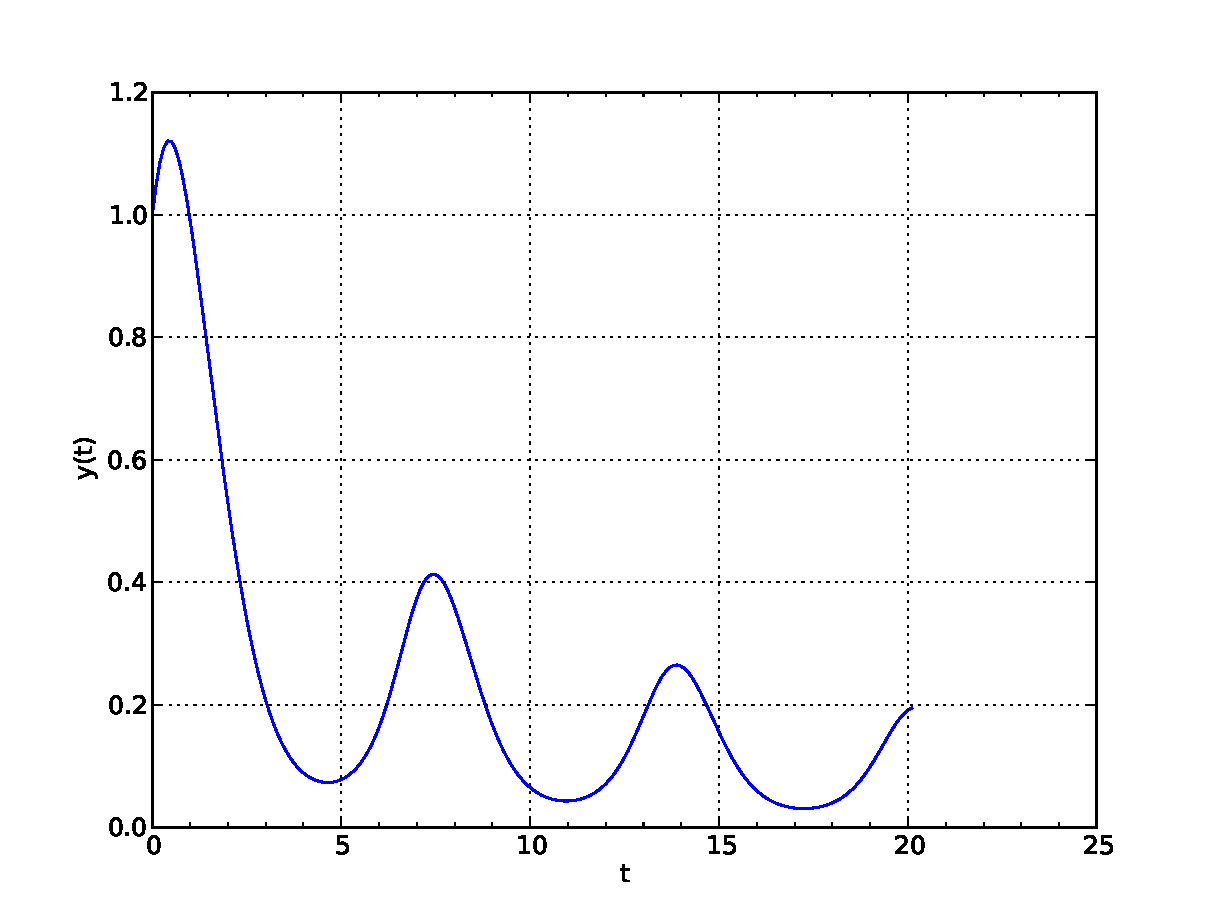
\includegraphics[width=0.65\linewidth]{grafica}
\end{center}
\caption{Representación gráfica de la función $y(t)$}
\label{fig:grafica}
\end{figure}
\end{document}